\documentclass[a4paper]{report}

\usepackage[utf8]{inputenc}
\usepackage[francais]{babel}
\usepackage[T1]{fontenc}
\usepackage[french,lined,boxed,commentsnumbered]{algorithm2e}
\usepackage{amsmath}
\usepackage{amsfonts}
\usepackage{amssymb}
\usepackage{placeins}
\usepackage{listings}
\usepackage{color}
\usepackage{textcomp}

%----- Package français
\usepackage[utf8]{inputenc} %reconnaissance des accents
\usepackage[francais]{babel} %document en français
\usepackage[T1]{fontenc} %codage des fonts TeX ?

%----- code ex: \BlankLine
\usepackage[french,lined,boxed,commentsnumbered]
{algorithm2e}


%----- math
\usepackage{amsmath}

%----- images
\usepackage{graphicx}

\title{Vérification formelle de site web\\premier rapport}
\author{Thomas BRIEN}
\date{6 Décembre 2012}

\begin{document}
\maketitle
\tableofcontents



\chapter*{Introduction}
\addcontentsline{toc}{chapter}{Introduction} 
Aujourd'hui, Internet est le moyen par excellence d'accéder à l'information. 
Il est donc essentiel de mettre en place des méthodes de vérification, afin d'assurer le bon fonctionnement des sites Web.\\



\chapter*{Définir un site WEB}
\addcontentsline{toc}{chapter}{Définir un site WEB}
\section{Les piliers du WEB\\}
\begin{tabbing}
1990' $ \Rightarrow$ \=$Hypertext Markup Language$ (HTML)\\
       \>$Hypertext Transfer Protocol$ (HTTP)\\
\end{tabbing}

\section{Composition d'un site\\}
On peut définir un site comme un ensemble de pages, ou documents, qui sont en fait des fichiers HTML. Ces documents sont reliés entre eux par des liens qu'on peut différencier en trois types:\\
\begin{itemize}
\item les liens entre deux documents du site
\item les liens internes à un document
\item les liens vers l extérieur
\end{itemize}

\section{Un exemple\\}
Prenons l'exemple simple d'un site hébergé à "monsite.com" et qui possède deux pages a.html et b.html.\\
La page a est constituée du code html suivant:\\
\begin{verbatim}
<html><body>
	<lu>
		<li><a href="http://google.fr">lien vers Google</a></li>
		<li><a href="b">aller à la page b</a></li>
		<li><a href="#monAncre">aller à l'ancre</a></li>
	</lu>
	<div id="monAncre"></div>
</body></html>
\end{verbatim}
Dans cet exemple, on a:
\begin{itemize}
\item un lien vers l’extérieur, qui renvoie vers google
\item un lien interne au site, de a vers b
\item un lien interne au document a.html
\end{itemize}

\chapter*{Définir un modèle pour les sites}
\addcontentsline{toc}{chapter}{Définir un modèle pour les sites}

\paragraph*{}
On a vu précédemment de quoi sont composés les sites web. Il est important à ce stade de modéliser les sites afin d'en retenir les propriétés essentielles et de permettre le traitement automatique de ces derniers. De par la structure du web (ensemble de pages liées entre elles), on devine que l'étude d'un site web pourra être ramenée à une étude de graph. On propose dans ce chapitre de décrire le graphe associé à un site.

\section{ Les nœuds du graphe (documents du site)\\ }
A chaque document du site, on fait correspondre un nœud N dans le graphe associé.
Par exemple, si on s'intéresse au document a.html décrit dans le chapitre précédant, on peux construire intuitivement un tuple contenant les informations essentielles au bon fonctionnement du site:
\begin{itemize}
\item l'URI du document: "http://monsite.com/a"
\item l'ancre: "monAncre"
\item le lien local: "$\#$monAncre"
\item le lien vers b: "b"
\item le lien externe: "http://www.google.fr"\\
\end{itemize}

Dans le cas général, on défini un nœud N du graphe comme suit: N = <u, lab, loc, site, ext, Sem>\\
 avec:\\
 $u$, l'URI associée à la page\\
 $lab$, la liste des "ancres" de la page\\
 $loc$, la liste des liens locaux dans la page\\
 $site$, la liste des liens internes du site définis dans la page\\
 $ext$, la liste des liens externes définis dans la page\\
 $Sem$, liste représentant les informations sémantiques relatives à la page.\\
 
\section{ Les liens entre documents\\ }
Une fois au point sur les annotations relatives à un nœud (un document) du site, on peut s'intéresser à l'expression des liens.\\
Soit un document $s = doc(m,h,u)$ qui pointe vers un autre document $d = doc(m,h,p)$ du site:\\
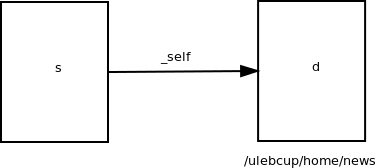
\includegraphics[scale=0.6]{lienSimple.png}\\
Un tel lien est représenté par un tuple <p, l, t>. Si le document s contient le lien html suivant:\\
<a href="/ulebcup/home/news"> News </a>\\
notre tuple devient: <p, l, t> = <"/ulebcup/home/news","", $\_$self> $\in$ site\\
$NB$: pour les liens externes, on doit re-préciser la méthode et l’hôte, de sorte que notre tuple sera enrichi comme suit: <m', h', p, l, t> = <"http","http://www.euroleague.net",
"/uleb/domestic-leagues","", $\_$blank>\\
\subsection*{ Les liens du graphe\\ }
On peut maintenant construire le graph associé au site en suivant les définitions données dans l'article (3.8 et 3.9)\\




\chapter*{ Vérification des propriétés du site }
\addcontentsline{toc}{chapter}{Vérification des propriétés du site}

\paragraph*{}
Une fois notre site correctement modélisé, on cherche à lui appliquer une logique de vérification afin de déterminer la présence ou l’absence de certaines propriétés. C'est le $model\ checking$.\\

\section*{La logique utilisée}
On utilise la logique LTL (Linear Temporal Logic).
Appliqué à une structure de Kripke

\section*{Vérification des propriétés sémantiques}





La vérification sera basée sur la logique LTL et appliquée à des structures de Kripke, comme défini en $page$ $9$.\\
\subsection*{ L'utilisation de la sémantique }
On s'appuie sur la sémantique des pages, de sorte que chaque élément de l'ensemble $Sem \mid_2$ peut être vu comme une propriété atomique. On peut par exemple écrire une formule qui vérifie que les pages privées ne sont pas accessibles directement depuis les pages publiques. On résonne sur $Sem$ = <"scope": \{public, private, access\}>: $\neg(public U private)$. En effet, on doit vérifier la propriété access avant de pouvoir vérifier private.\\


\chapter*{ Extensions souhaitables: }

\begin{itemize}
\item au niveau du langage (pas seulement html)
\item au niveau de la quantification du temps en LTL
\end{itemize}

\end{document}